\section{Pebble Bed Solid Breeder Blanket Concepts}\label{sec:blanket-design}

\begin{figure}
	\centering
	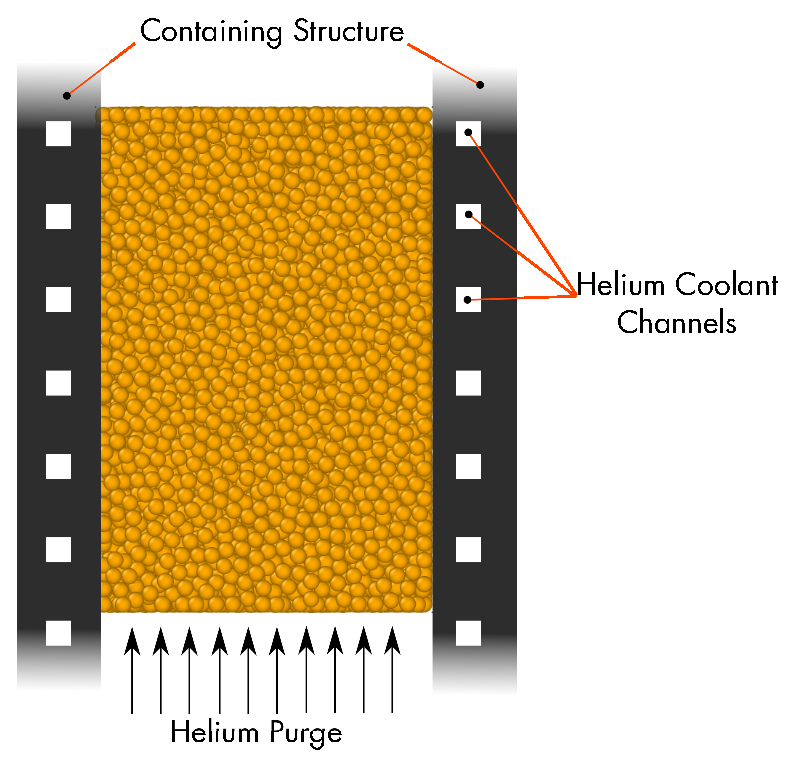
\includegraphics[width=0.85\textwidth]{chapters/figures/solid_breeder_sketch} 
	\caption{Sketch of a typical unit of a pebble bed tritium breeding zone. The pebble bed is cooled with contact to the containing structure.}
	\label{fig:solid-breeder-sketch}
\end{figure}

Figure~\ref{fig:solid-breeder-sketch} is a sketch showing many of the important physical features of lithium ceramic pebble bed in a solid breeder. In typical solid breeder modules, a high pressure helium coolant runs through the containing structure of ferritic or austenitic steel surrounding the pebble bed; the coolant will heat to approximately 500~\celsius before exiting the blanket. A low-pressure, low-speed purge gas is pumped through the pebble bed to extract the tritium generated and transport it out of the blanket for processing. 

In addition to breeding tritium, the blanket will be responsible for power extraction in the fusion reactor. The blanket must function to capture the kinetic energy of neutrons (80\% of the fusion energy is carried by the neutron), secondary $\gamma$ rays, and the surface radiation on the plasma-facing first wall (an integral component with the blanket). The blanket must also be able to convert the fusion's energy into high quality heat that can be extracted into the power cycle connected to the fusion reactor. 

The dual role of the breeding blanket to generate heat and tritium forces a specific operational temperature window for the ceramic pebble beds. The low end of the temperature window is governed by a minimum temperature for acceptable release rates of tritium from the ceramic to the purge gas; the value is generally set around 300~\celsius. The upper limit of the temperature window is chosen to avoid sintering of the lithiated ceramic. Tritium that transmutes from the lithium inside the pebble must diffuse slowly through the bulk until reaching a grain boundary. Tritium moves relatively quickly along the grain boundary until reaching a surface of open porosity where it may desorb into the passing purge gas.\cite{Federici1990} Based on this understanding of tritium release from the pebble, sintering of the ceramics, as grains in individual pebbles merge, is predicted to reduce the rate of tritium release. The upper end of the temperature window is therefore generally set around 900~\celsius.

The size of breeder region is limited by the operational temperature window that must be held in spite of the the poor effective conductivity of packed beds of ceramic pebbles. The conductivity is experimentally shown to be a weak function of external pressure but can generally no greater than about \si{1 W/{mK}} -- for well-packed beds. Because the effective conductivity and packed bed-wall interface conductance is predominately a contact conduction, disruptions to the packing structure will have considerable impact on the heat transfer of the packed bed.

Moreover, as nuclear energy is deposited into the poorly-conductive ceramic breeder material and the temperature climbs well above the containing structure, it will confine the thermal expansion of the lithium ceramic and lead to mechanical stresses at the points of contact of the individual pebbles in the packed bed. Engineering design issues surrounding this thermally-induced stress is of great concern to researchers and will be the focus of much of this report.





 % the fusion reaction deposits   The nuclear heat generated in the pebble bed solid breeder will heat the ceramic pebbles to maximum temperatures of approximately 900~\celsius. The heat of the pebbles is transported through them via conduction through inter-particle contacts, conduction through the purge gas into neighboring particles, and ultimately through contact with the containing structure. The box structure surrounding the solid breeder will have high pressure (\si{8~MPa} in many current designs) 